\documentclass[12pt,a4paper]{article}
\usepackage[margin=1in]{geometry}
\usepackage[T1]{fontenc}
\usepackage[utf8]{inputenc}
\usepackage{hyperref}
\usepackage{longtable}
\usepackage{array}
\usepackage{enumitem}
\usepackage{xcolor}
\usepackage{listings}
\usepackage{titlesec}
\usepackage{tikz}
\usetikzlibrary{arrows.meta, positioning, shapes.geometric}

\hypersetup{
    colorlinks=true,
    linkcolor=blue,
    urlcolor=blue
}

\lstdefinestyle{plaincode}{
    basicstyle=\ttfamily\small,
    breaklines=true,
    frame=single,
    columns=fullflexible
}

\tikzset{
    flowbox/.style={
        rectangle,
        rounded corners,
        draw=black,
        align=center,
        minimum width=3.2cm,
        minimum height=1cm,
        fill=blue!5
    },
    flowdecision/.style={
        diamond,
        draw=black,
        align=center,
        aspect=2,
        inner sep=1pt,
        fill=orange!10
    },
    flowline/.style={
        -{Latex[length=2.5mm]},
        thick
    }
}

\titleformat{\section}{\large\bfseries}{\thesection}{0.75em}{}
\titleformat{\subsection}{\normalsize\bfseries}{\thesubsection}{0.75em}{}

\title{GramExpress Project Documentation}
\author{Repository Documentation Source}
\date{April 4, 2026}

\begin{document}
\maketitle
\tableofcontents
\newpage

\section{Introduction}
GramExpress is a mobile-first Django application that models a hyperlocal delivery workflow for three primary business roles: customer, store owner, and rider. The repository is implemented as a server-rendered web application, not as a split frontend and backend monorepo. Django handles the application logic, templating, static asset delivery in development, authentication, and database access.

This document is provided in LaTeX source format only. It is intended to describe the complete current project as represented in the repository, including architecture, module layout, domain model, authentication flows, checkout and delivery flows, configuration, seeded data, and test coverage.

\section{Project Goals}
The system is designed to demonstrate the core capabilities of a local commerce and last-mile delivery platform:
\begin{itemize}[leftmargin=1.5em]
    \item unified account access using phone or email;
    \item OTP-assisted registration and login flows;
    \item distinct dashboards for customer, shop owner, and rider roles;
    \item product browsing, session cart management, and checkout;
    \item order tracking, rider handoff OTP, and delivery completion;
    \item notification-driven user updates;
    \item an installable progressive web app shell for mobile usage.
\end{itemize}

\section{Technology Stack}
\begin{longtable}{|p{0.28\linewidth}|p{0.62\linewidth}|}
\hline
\textbf{Layer} & \textbf{Implementation} \\
\hline
Backend framework & Django 5.2.x \\
\hline
Language & Python 3.11 \\
\hline
Database & SQLite for local development \\
\hline
Frontend & Django templates with custom CSS \\
\hline
Static assets & \texttt{static/core/} \\
\hline
Authentication & Django auth plus custom role-profile mapping \\
\hline
OTP delivery & Email backend and SMS backend with console or Twilio option \\
\hline
Payments & COD flow plus Razorpay-related checkout and settlement fields \\
\hline
PWA support & Manifest endpoint and service worker endpoint \\
\hline
\end{longtable}

\section{Repository Structure}
The repository is centered around one Django project package and one main app package:

\begin{lstlisting}[style=plaincode]
gramexpress/
|- manage.py
|- requirements.txt
|- README.md
|- core/
|  |- admin.py
|  |- apps.py
|  |- context_processors.py
|  |- forms.py
|  |- models.py
|  |- tests.py
|  |- urls.py
|  |- views.py
|  |- management/commands/seed_demo.py
|  `- migrations/
|- gramexpress/
|  |- settings.py
|  |- urls.py
|  |- asgi.py
|  `- wsgi.py
|- templates/core/
`- static/core/
\end{lstlisting}

\subsection{High-Level Responsibilities}
\begin{itemize}[leftmargin=1.5em]
    \item \texttt{gramexpress/settings.py} defines the runtime configuration, environment-variable loading, installed apps, middleware, and storage settings.
    \item \texttt{core/models.py} contains the business data model and the domain enums used throughout the system.
    \item \texttt{core/views.py} contains nearly all application behavior, including authentication, cart logic, checkout, order state changes, notifications, and PWA endpoints.
    \item \texttt{core/forms.py} defines styled forms for login, OTP verification, registration, profile updates, products, ratings, and rider location updates.
    \item \texttt{core/urls.py} exposes the route map for customer, shop, rider, payment, support, and notification workflows.
    \item \texttt{templates/core/} contains the server-rendered user interface for all roles.
    \item \texttt{static/core/styles.css} provides the main visual styling.
    \item \texttt{core/management/commands/seed\_demo.py} creates demo accounts and sample data for local use.
\end{itemize}

\section{Runtime Architecture}
\subsection{Application Pattern}
GramExpress follows a classic Django server-rendered architecture:
\begin{enumerate}[leftmargin=1.5em]
    \item the browser requests a page or submits a form;
    \item Django routes the request through \texttt{gramexpress/urls.py} and \texttt{core/urls.py};
    \item view functions in \texttt{core/views.py} perform validation, read or mutate model data, and prepare context;
    \item Django renders templates in \texttt{templates/core/};
    \item static assets are served locally during development;
    \item SQLite stores all relational data in \texttt{db.sqlite3}.
\end{enumerate}

\subsection{Role-Aware Behavior}
The application is role-aware at the business-model layer rather than by relying only on the built-in Django groups system. A Django user can be associated with one of several profile models:
\begin{itemize}[leftmargin=1.5em]
    \item \texttt{CustomerProfile}
    \item \texttt{ShopOwnerProfile}
    \item \texttt{RiderProfile}
\end{itemize}

This approach lets the code attach role-specific data, dashboard behavior, and workflows while still using Django's native session authentication.

\section{Configuration}
\subsection{Environment Loading}
The project loads environment variables from a local \texttt{.env} file via \texttt{python-dotenv}. This file is read from the project base directory during Django startup.

\subsection{Core Settings}
Important settings in the current codebase include:
\begin{itemize}[leftmargin=1.5em]
    \item \texttt{DEBUG}
    \item \texttt{SECRET\_KEY}
    \item \texttt{ALLOWED\_HOSTS}
    \item \texttt{CSRF\_TRUSTED\_ORIGINS}
    \item SQLite database configuration
    \item static and media path configuration
    \item login and redirect URLs
    \item OTP expiry duration
    \item email backend configuration
    \item SMS backend configuration
    \item Google sign-in configuration
    \item Google Maps keys
    \item Razorpay payment and settlement configuration
\end{itemize}

\subsection{Environment Variables Used by the Code}
\begin{longtable}{|p{0.36\linewidth}|p{0.54\linewidth}|}
\hline
\textbf{Variable} & \textbf{Purpose} \\
\hline
\texttt{SECRET\_KEY} & Django application secret key \\
\hline
\texttt{DEBUG} & Development mode toggle \\
\hline
\texttt{GRAMEXPRESS\_APP\_NAME} & Branding label used by the application \\
\hline
\texttt{GOOGLE\_MAPS\_BROWSER\_API\_KEY} & Browser-side maps integration \\
\hline
\texttt{GOOGLE\_MAPS\_EMBED\_API\_KEY} & Embedded maps integration \\
\hline
\texttt{GOOGLE\_CLIENT\_ID} & Google sign-in token audience validation \\
\hline
\texttt{RAZORPAY\_KEY\_ID} & Razorpay payment integration key \\
\hline
\texttt{RAZORPAY\_KEY\_SECRET} & Razorpay secret key \\
\hline
\texttt{RAZORPAY\_WEBHOOK\_SECRET} & Razorpay webhook verification secret \\
\hline
\texttt{RAZORPAY\_SETTLEMENT\_QR\_IMAGE\_URL} & QR image used for COD settlement flow \\
\hline
\texttt{RAZORPAY\_SETTLEMENT\_UPI\_ID} & UPI target for settlement collection \\
\hline
\texttt{DEFAULT\_FROM\_EMAIL} & Sender for email notifications and OTP \\
\hline
\texttt{EMAIL\_BACKEND} & Email delivery backend \\
\hline
\texttt{EMAIL\_HOST}, \texttt{EMAIL\_PORT}, \texttt{EMAIL\_HOST\_USER}, \texttt{EMAIL\_HOST\_PASSWORD}, \texttt{EMAIL\_USE\_TLS} & SMTP configuration \\
\hline
\texttt{OTP\_EXPIRY\_MINUTES} & Expiry window for auth OTPs \\
\hline
\texttt{SMS\_BACKEND} & SMS delivery mode, including console or Twilio \\
\hline
\texttt{SMS\_FROM} & Sender number for Twilio SMS \\
\hline
\texttt{TWILIO\_ACCOUNT\_SID}, \texttt{TWILIO\_AUTH\_TOKEN} & Twilio credentials \\
\hline
\end{longtable}

\section{Domain Model}
\subsection{Reference Enums}
The code defines several \texttt{TextChoices} enums that shape business behavior:
\begin{itemize}[leftmargin=1.5em]
    \item \texttt{ApprovalStatus}: pending, approved, rejected
    \item \texttt{ShopType}: kirana, medical, bakery
    \item \texttt{VehicleType}: electric, petrol
    \item \texttt{OrderStatus}: pending, confirmed, packed, out\_for\_delivery, delivered, cancelled
    \item \texttt{PaymentMethod}: COD, Razorpay
    \item \texttt{PaymentStatus}: pending, paid, failed
    \item \texttt{CodCollectionMode}: online, cash
    \item \texttt{SettlementStatus}: not\_required, qr\_ready, paid, failed
    \item \texttt{RoleType}: customer, shop, rider, admin
    \item \texttt{NotificationType}: order, store, rider, payment, promo, system
    \item \texttt{OtpPurpose}: register, login\_email
    \item \texttt{OtpChannel}: email, SMS
\end{itemize}

\subsection{Abstract Models}
\subsubsection{TimeStampedModel}
Provides \texttt{created\_at} and \texttt{updated\_at}. Many business objects inherit from this base so the system can group notifications, order timelines, and recent activity by time.

\subsubsection{LocationMixin}
Provides:
\begin{itemize}[leftmargin=1.5em]
    \item latitude;
    \item longitude;
    \item a computed Google Maps search URL;
    \item a short coordinate string representation.
\end{itemize}

\subsection{Primary Business Models}
\subsubsection{CustomerProfile}
Stores the customer-specific identity and delivery details:
\begin{itemize}[leftmargin=1.5em]
    \item linked Django user;
    \item full name, phone, and email;
    \item preferred language;
    \item address lines, district, and pincode;
    \item latitude and longitude.
\end{itemize}

\subsubsection{ShopOwnerProfile}
Represents a store owner:
\begin{itemize}[leftmargin=1.5em]
    \item linked Django user;
    \item full name, phone, and email;
    \item approval status for moderation.
\end{itemize}

\subsubsection{RiderProfile}
Represents a delivery rider:
\begin{itemize}[leftmargin=1.5em]
    \item linked Django user;
    \item full name, phone, and email;
    \item age and vehicle type;
    \item approval status;
    \item availability flag;
    \item service radius and maximum service radius;
    \item rating;
    \item coordinates;
    \item optional photo URL or uploaded file.
\end{itemize}

\subsubsection{Shop}
Represents a merchant storefront:
\begin{itemize}[leftmargin=1.5em]
    \item owner foreign key;
    \item shop name and auto-generated slug;
    \item shop type;
    \item service area and address;
    \item descriptive text and offer label;
    \item image URL or uploaded image;
    \item open or closed state;
    \item approval status;
    \item rating;
    \item coordinates.
\end{itemize}

\subsubsection{Product}
Represents a sellable item associated with a shop:
\begin{itemize}[leftmargin=1.5em]
    \item product name and subtitle;
    \item category and unit;
    \item price and stock;
    \item image URL;
    \item decorative color value;
    \item merchandising tag.
\end{itemize}

\subsubsection{CheckoutSession}
Captures the state of a checkout attempt before or while orders are finalized:
\begin{itemize}[leftmargin=1.5em]
    \item customer;
    \item payment method and payment status;
    \item amount and currency;
    \item customer notes and delivery address;
    \item cart snapshot and cart signature;
    \item receipt and Razorpay identifiers;
    \item failure reason;
    \item completion timestamp.
\end{itemize}

\subsubsection{Order}
This is the central transactional model. It stores:
\begin{itemize}[leftmargin=1.5em]
    \item customer, shop, rider, and checkout session references;
    \item current lifecycle status;
    \item payment method, payment status, and payment reference;
    \item COD collection mode and COD payment link metadata;
    \item customer payment timestamp and cash confirmation timestamp;
    \item settlement state and settlement-related fields;
    \item total amount and delivery fee;
    \item delivery address and customer notes;
    \item delivery OTP for handoff;
    \item cancellation metadata;
    \item customer and store rating fields;
    \item delivery completion timestamp.
\end{itemize}

The model also exposes behavior such as recalculating totals, generating a display ID, reporting tracking labels, and checking cancellation or rating eligibility.

\subsubsection{OrderItem}
Connects an order to a product and stores:
\begin{itemize}[leftmargin=1.5em]
    \item quantity;
    \item unit price at the time of order;
    \item computed line total.
\end{itemize}

\subsubsection{Notification}
Stores role-targeted notifications with:
\begin{itemize}[leftmargin=1.5em]
    \item optional customer target;
    \item optional shop owner target;
    \item optional rider target;
    \item optional related order;
    \item notification type;
    \item title and body;
    \item read or unread state.
\end{itemize}

\subsubsection{EmailOtpToken}
This model represents an earlier email OTP workflow and remains in the codebase for compatibility and continuity.

\subsubsection{AuthOtpToken}
This is the main OTP model used by the current authentication flows. It stores:
\begin{itemize}[leftmargin=1.5em]
    \item linked user when available;
    \item role;
    \item OTP purpose;
    \item delivery channel;
    \item email or phone target;
    \item 6-digit OTP code;
    \item expiration timestamp;
    \item used flag;
    \item metadata JSON for flow-specific state.
\end{itemize}

\section{Authentication and Identity Design}
\subsection{User Resolution}
The application resolves identities by phone number or email address. Instead of treating the Django username as the only entry point, it searches the profile tables to determine whether the supplied identity maps to a customer, shop owner, or rider. This is important because role drives both dashboard routing and authorization behavior.

\subsection{Login Paths}
The system supports two major login paths:
\begin{enumerate}[leftmargin=1.5em]
    \item phone or email plus password through the standard login view;
    \item passwordless email OTP through the email OTP flow.
\end{enumerate}

When email-based login is used, the system can require OTP completion before granting full access.

\subsection{Registration Path}
The registration flow is unified into one role-aware form. The selected account type controls which fields are required. Customer registration captures address and language, shop registration captures shop metadata, and rider registration captures vehicle and location details. Registration includes mobile OTP verification before the account is finalized.

\subsection{Google Sign-In}
The code includes a Google sign-in verification hook. It validates the Google credential token against the configured Google client ID, then allows the application to connect existing accounts. This is not a full standalone OAuth implementation with dedicated social-auth persistence.

\section{Forms Layer}
\subsection{Design}
The forms layer is responsible for validation, field styling, and role-aware required fields. A shared \texttt{BaseStyledForm} injects consistent input classes and useful HTML attributes such as placeholder text, autocomplete hints, and mobile-friendly input modes.

\subsection{Important Forms}
\begin{longtable}{|p{0.34\linewidth}|p{0.56\linewidth}|}
\hline
\textbf{Form} & \textbf{Purpose} \\
\hline
\texttt{LoginForm} & Identity and password login \\
\hline
\texttt{LoginOtpVerifyForm} & Email OTP verification after login \\
\hline
\texttt{EmailOtpRequestForm} & Passwordless email OTP request \\
\hline
\texttt{EmailOtpVerifyForm} & Passwordless email OTP verification \\
\hline
\texttt{UnifiedRegistrationForm} & Role-aware registration for customer, shop, and rider \\
\hline
\texttt{CustomerProfileForm} & Customer profile updates \\
\hline
\texttt{ShopUpdateForm} & Shop metadata updates \\
\hline
\texttt{ProductForm} & Product creation and editing \\
\hline
\texttt{CustomerOrderMetaForm} & Payment method and checkout notes \\
\hline
\texttt{RatingForm} & Customer rating of an order \\
\hline
\texttt{StoreRatingForm} & Store rating of a rider delivery \\
\hline
\texttt{RiderLocationForm} & Rider coordinate updates \\
\hline
\end{longtable}

\section{Routing and Functional Areas}
\subsection{Project URL Configuration}
The top-level URL configuration is intentionally minimal:
\begin{itemize}[leftmargin=1.5em]
    \item \texttt{/admin/} for Django admin;
    \item all remaining routes are delegated to \texttt{core.urls}.
\end{itemize}

\subsection{Main Route Groups}
\begin{longtable}{|p{0.28\linewidth}|p{0.62\linewidth}|}
\hline
\textbf{Route Group} & \textbf{Purpose} \\
\hline
\texttt{/auth/...} & login, registration, Google auth, and email OTP \\
\hline
\texttt{/customer/...} & customer dashboard, cart, checkout, orders, profile, and order actions \\
\hline
\texttt{/shop/...} & shop dashboard, products, settings, and order state transitions \\
\hline
\texttt{/rider/...} & rider dashboard, deliveries, availability, location, and handoff actions \\
\hline
\texttt{/notifications/...} & notification list, read state changes, and linked navigation \\
\hline
\texttt{/orders/...} & order detail and tracking views \\
\hline
\texttt{/payments/...} & Razorpay webhook handler \\
\hline
\texttt{/manifest.json} and \texttt{/service-worker.js} & PWA endpoints \\
\hline
\end{longtable}

\section{Major User Workflows}
\subsection{Customer Workflow}
The customer journey is built around discovery, checkout, and tracking:
\begin{enumerate}[leftmargin=1.5em]
    \item authenticate or register;
    \item browse approved and open shops;
    \item inspect store details and products;
    \item add items to the session cart;
    \item review cart and checkout details;
    \item choose payment method;
    \item create order records;
    \item receive order and rider notifications;
    \item view order detail and tracking;
    \item confirm COD cash when applicable;
    \item reorder or rate completed deliveries.
\end{enumerate}

\subsection{Shop Workflow}
The store owner workflow is centered on catalog management and order processing:
\begin{enumerate}[leftmargin=1.5em]
    \item authenticate as a store owner;
    \item access the store dashboard;
    \item manage store settings and basic metadata;
    \item create, edit, and remove products;
    \item review incoming orders;
    \item update order status from pending toward dispatch;
    \item monitor rider assignment and delivery progress;
    \item rate rider performance after delivery.
\end{enumerate}

\subsection{Rider Workflow}
The rider workflow combines availability, dispatch acceptance, and proof-of-handoff:
\begin{enumerate}[leftmargin=1.5em]
    \item authenticate as an approved rider;
    \item toggle availability;
    \item inspect delivery queue and assigned work;
    \item accept an eligible order;
    \item update rider location;
    \item confirm pickup when near the shop geofence;
    \item send or resend delivery OTP reminders;
    \item complete delivery after verifying the customer OTP;
    \item return to available status after completion.
\end{enumerate}

\subsection{Notification Workflow}
Notifications are created for all three major roles and are displayed in a dedicated notification center. Users can:
\begin{itemize}[leftmargin=1.5em]
    \item view grouped notifications;
    \item mark a single notification as read;
    \item mark all notifications as read;
    \item open a notification and navigate to the relevant screen.
\end{itemize}

\section{System Flowchart}
The following flowchart summarizes the main end-to-end interaction across authentication, ordering, fulfillment, and completion:

\begin{figure}[h!]
\centering
\resizebox{\textwidth}{!}{
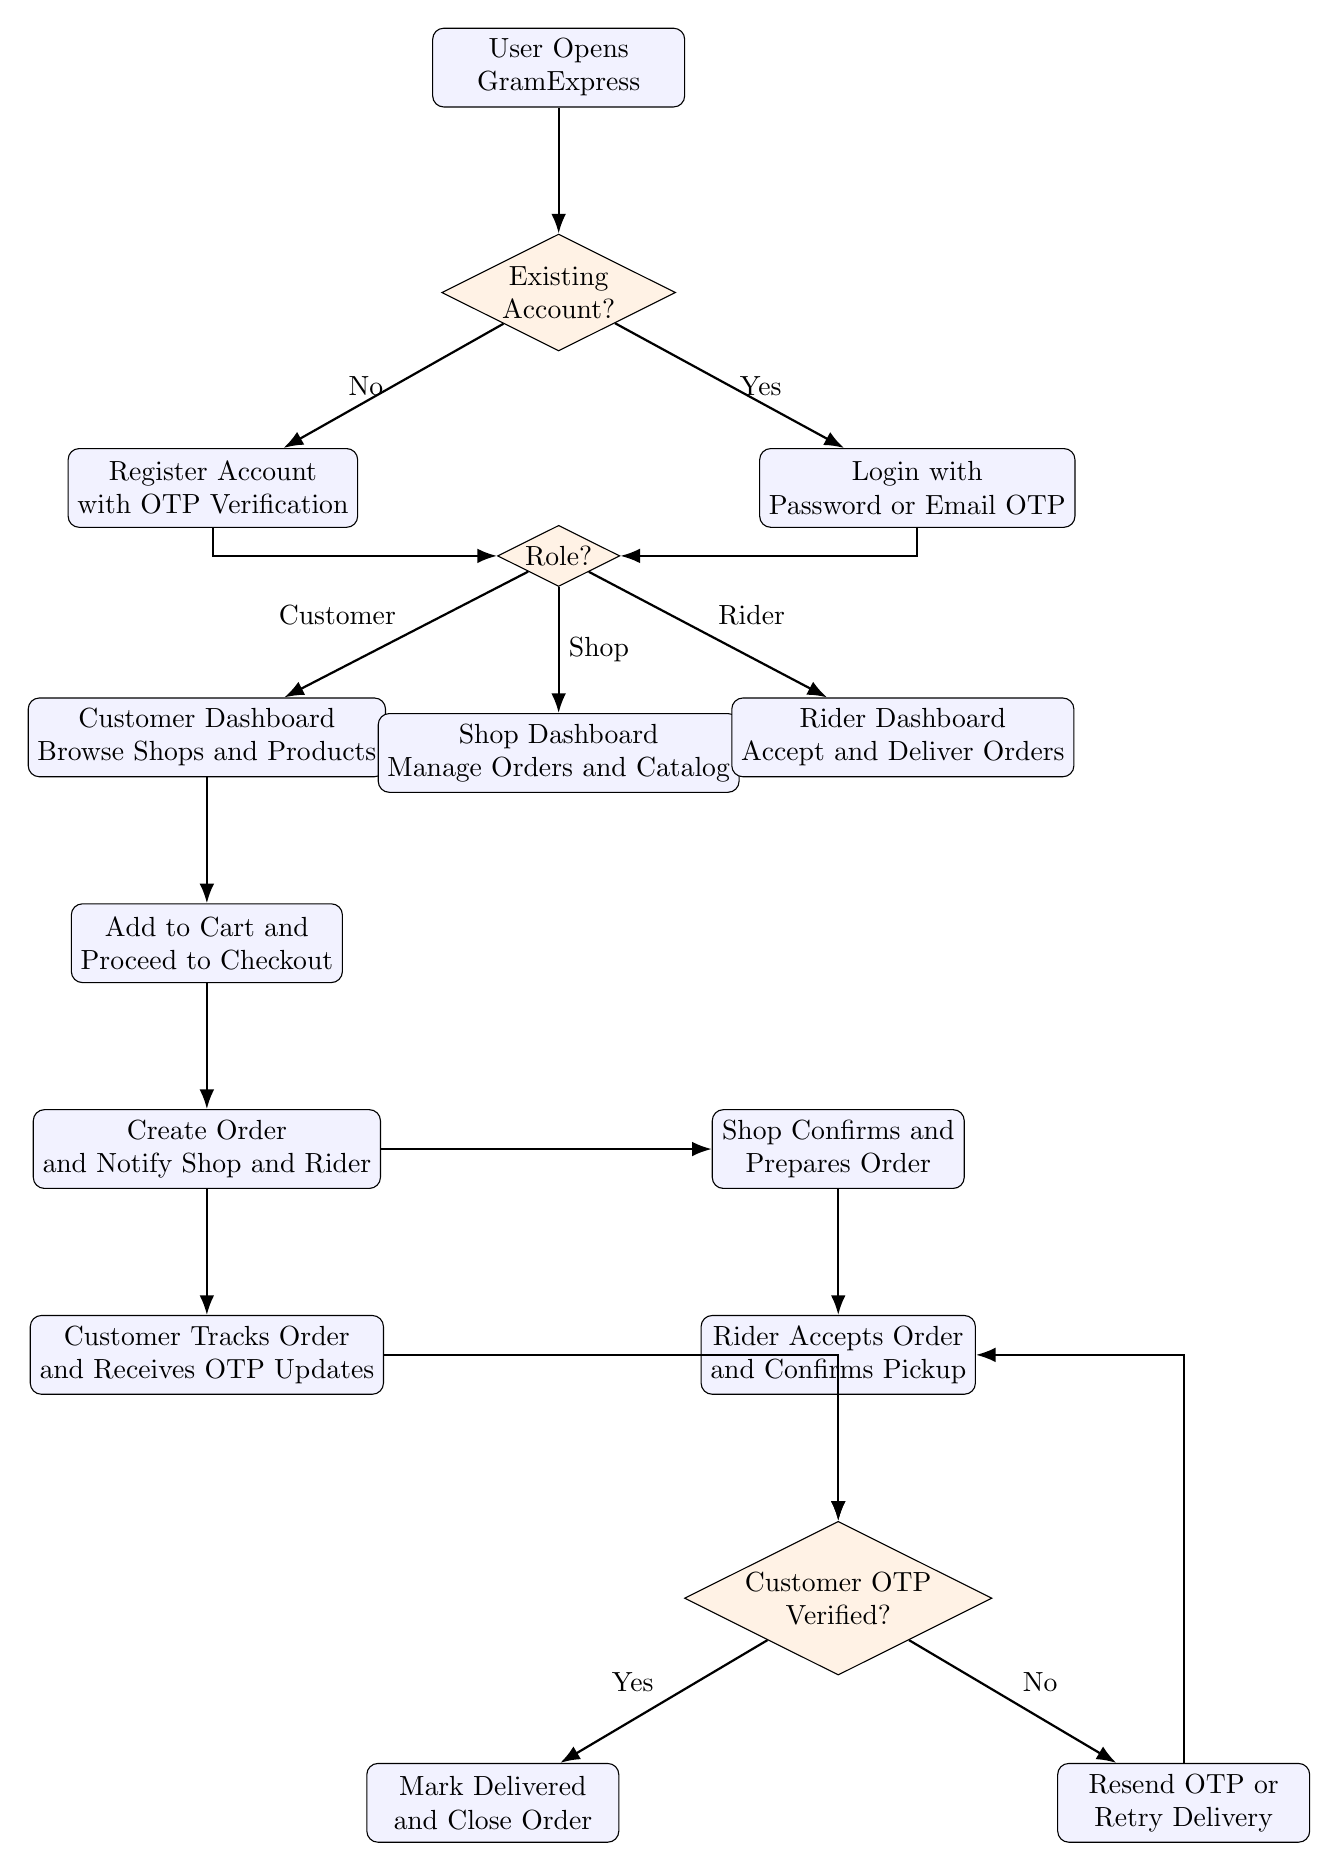
\begin{tikzpicture}[node distance=1.6cm and 1.8cm]
    \node[flowbox] (start) {User Opens\\GramExpress};
    \node[flowdecision, below=of start] (auth) {Existing\\Account?};
    \node[flowbox, below left=of auth] (register) {Register Account\\with OTP Verification};
    \node[flowbox, below right=of auth] (login) {Login with\\Password or Email OTP};
    \node[flowdecision, below=2.2cm of auth] (role) {Role?};

    \node[flowbox, below left=of role] (customer) {Customer Dashboard\\Browse Shops and Products};
    \node[flowbox, below=of role] (shop) {Shop Dashboard\\Manage Orders and Catalog};
    \node[flowbox, below right=of role] (rider) {Rider Dashboard\\Accept and Deliver Orders};

    \node[flowbox, below=of customer] (cart) {Add to Cart and\\Proceed to Checkout};
    \node[flowbox, below=of cart] (order) {Create Order\\and Notify Shop and Rider};
    \node[flowbox, right=4.2cm of order] (prepare) {Shop Confirms and\\Prepares Order};
    \node[flowbox, below=of prepare] (pickup) {Rider Accepts Order\\and Confirms Pickup};
    \node[flowbox, below=of order] (track) {Customer Tracks Order\\and Receives OTP Updates};
    \node[flowdecision, below=of pickup] (handoff) {Customer OTP\\Verified?};
    \node[flowbox, below left=of handoff] (delivered) {Mark Delivered\\and Close Order};
    \node[flowbox, below right=of handoff] (resend) {Resend OTP or\\Retry Delivery};

    \draw[flowline] (start) -- (auth);
    \draw[flowline] (auth) -- node[left] {No} (register);
    \draw[flowline] (auth) -- node[right] {Yes} (login);
    \draw[flowline] (register) |- (role);
    \draw[flowline] (login) |- (role);

    \draw[flowline] (role) -- node[above left] {Customer} (customer);
    \draw[flowline] (role) -- node[right] {Shop} (shop);
    \draw[flowline] (role) -- node[above right] {Rider} (rider);

    \draw[flowline] (customer) -- (cart);
    \draw[flowline] (cart) -- (order);
    \draw[flowline] (order) -- (track);
    \draw[flowline] (order) -- (prepare);
    \draw[flowline] (prepare) -- (pickup);
    \draw[flowline] (pickup) -- (handoff);
    \draw[flowline] (track) -| (handoff);
    \draw[flowline] (handoff) -- node[above left] {Yes} (delivered);
    \draw[flowline] (handoff) -- node[above right] {No} (resend);
    \draw[flowline] (resend) |- (pickup);
\end{tikzpicture}
}
\caption{High-level GramExpress workflow from authentication to delivery completion}
\end{figure}

\section{Checkout, Payment, and Delivery Logic}
\subsection{Cart Handling}
Cart state is session-based rather than persisted as a dedicated cart model. This keeps the demo lightweight while still enabling:
\begin{itemize}[leftmargin=1.5em]
    \item adding products;
    \item updating quantities;
    \item clearing the cart;
    \item validating stock before checkout.
\end{itemize}

\subsection{Checkout Session}
Before or during order creation, the application captures a checkout session snapshot. This structure supports:
\begin{itemize}[leftmargin=1.5em]
    \item customer checkout review;
    \item cart signature tracking;
    \item payment outcome linking;
    \item retry and failure visibility.
\end{itemize}

\subsection{Order Lifecycle}
The main order state machine consists of:
\begin{enumerate}[leftmargin=1.5em]
    \item \texttt{pending}
    \item \texttt{confirmed}
    \item \texttt{packed}
    \item \texttt{out\_for\_delivery}
    \item \texttt{delivered}
    \item \texttt{cancelled}
\end{enumerate}

The customer can cancel only in eligible early states. Riders can move a qualifying order into pickup and then delivery-complete states. The final handoff requires OTP verification.

\subsection{COD and Razorpay Support}
The codebase includes support for:
\begin{itemize}[leftmargin=1.5em]
    \item COD as a primary payment method;
    \item Razorpay-related checkout completion and failure endpoints;
    \item COD online payment link support;
    \item settlement metadata for post-delivery reconciliation.
\end{itemize}

This indicates a hybrid payment design where delivery and settlement can be tracked more deeply than a simple cash-or-online toggle.

\subsection{Delivery OTP}
Customer handoff OTP is a central trust mechanism in the delivery flow:
\begin{itemize}[leftmargin=1.5em]
    \item a delivery OTP is stored per order;
    \item riders can resend a fresh OTP reminder under cooldown rules;
    \item delivery completion checks OTP validity and equality before accepting the handoff;
    \item the system also accounts for OTP expiry.
\end{itemize}

\section{OTP Delivery and Messaging}
\subsection{Email OTP}
Email OTP messages are sent using Django's email backend. In local development, the console email backend can be used so the OTP is printed directly in the server terminal instead of being sent to a real mailbox.

\subsection{SMS OTP}
SMS OTP delivery supports two modes:
\begin{itemize}[leftmargin=1.5em]
    \item console mode, where the OTP is printed to the server output;
    \item Twilio mode, where an HTTP request is made to Twilio's message API.
\end{itemize}

\subsection{Operational Implication}
With the console backends enabled, local testing becomes simple because both email OTP and mobile OTP can be retrieved directly from the terminal where \texttt{runserver} is running.

\section{Templates and Frontend Composition}
\subsection{Rendering Approach}
The frontend is not a separate JavaScript application. Instead, the project uses Django templates for all views. This means the backend and frontend are delivered together by the same Django server process.

\subsection{Template Coverage}
The repository includes dedicated templates for:
\begin{itemize}[leftmargin=1.5em]
    \item home and login pages;
    \item registration and email OTP screens;
    \item customer dashboard, cart, profile, orders, checkout review, and checkout success;
    \item shop dashboard, products, orders, settings, and start page;
    \item rider dashboard, deliveries, completed orders, earnings, profile, and start page;
    \item order detail and order tracking;
    \item notifications and support;
    \item a tailwind-theme reference page.
\end{itemize}

\subsection{Styling}
Primary styling is maintained in \texttt{static/core/styles.css}. The codebase also includes app icons and reference images used by the UI and progressive web app shell.

\section{Progressive Web App Support}
The application exposes two PWA endpoints:
\begin{itemize}[leftmargin=1.5em]
    \item \texttt{/manifest.json}
    \item \texttt{/service-worker.js}
\end{itemize}

The service worker caches shell assets and supports installation-oriented mobile usage. Asset versioning is derived from file modification times of selected template and static files, which helps invalidate stale shell caches during development changes.

\section{Seed Data}
\subsection{Purpose}
The \texttt{seed\_demo} management command creates a consistent local environment for demonstrations and testing. This is important because the application has multiple roles and workflows that are difficult to inspect without prepared data.

\subsection{Objects Created}
The seed script creates or refreshes:
\begin{itemize}[leftmargin=1.5em]
    \item an admin user;
    \item a customer user and profile;
    \item a store owner user and profile;
    \item a rider user and profile;
    \item an approved shop;
    \item sample products;
    \item a sample order and order items;
    \item starter notifications.
\end{itemize}

\subsection{Demo Credentials}
The repository documentation and seed logic establish the following demo access:
\begin{itemize}[leftmargin=1.5em]
    \item Admin: \texttt{admin / admin123}
    \item Customer phone: \texttt{+919188843299}
    \item Store phone: \texttt{+919900010101}
    \item Rider phone: \texttt{+919900011111}
    \item Shared non-admin password: \texttt{demo12345}
\end{itemize}

\section{Database and Migrations}
\subsection{Database Choice}
The local environment uses SQLite, configured through Django's default database connection. This means there is no separate database server process to launch during development.

\subsection{Migration History}
The current migration sequence in the repository is:
\begin{enumerate}[leftmargin=1.5em]
    \item \texttt{0001\_initial}
    \item \texttt{0002\_customerprofile\_user\_order\_customer\_rating\_and\_more}
    \item \texttt{0003\_authotptoken}
    \item \texttt{0004\_order\_cancellation\_reason\_order\_cancelled\_by\_role}
    \item \texttt{0005\_notification\_notification\_type}
    \item \texttt{0006\_checkoutsession\_order\_checkout\_session}
    \item \texttt{0007\_order\_cash\_confirmed\_at\_order\_cod\_collection\_mode\_and\_more}
\end{enumerate}

The migration chain shows the project evolving from a simpler transactional core into a richer workflow with OTP, notifications, checkout sessions, COD handling, and settlement support.

\section{Testing}
\subsection{Test Coverage Themes}
The repository includes \texttt{core/tests.py}, which exercises important behavior such as:
\begin{itemize}[leftmargin=1.5em]
    \item login and registration rendering;
    \item role-based redirects;
    \item cart and checkout operations;
    \item stock validation;
    \item notifications;
    \item order detail and tracking;
    \item cancellation and reorder behavior;
    \item registration OTP flow;
    \item email OTP flow;
    \item admin approval behavior;
    \item delivery OTP reminders and expiry handling.
\end{itemize}

\subsection{Testing Command}
\begin{lstlisting}[style=plaincode]
python manage.py test
\end{lstlisting}

\section{Local Setup and Run Instructions}
\subsection{Initial Setup}
\begin{lstlisting}[style=plaincode]
python -m venv .venv
.venv\Scripts\python -m pip install -r requirements.txt
Copy-Item .env.example .env
.venv\Scripts\python manage.py migrate
.venv\Scripts\python manage.py seed_demo
\end{lstlisting}

\subsection{Run the Development Server}
\begin{lstlisting}[style=plaincode]
.venv\Scripts\python manage.py runserver 0.0.0.0:8000
\end{lstlisting}

Then open:
\begin{lstlisting}[style=plaincode]
http://127.0.0.1:8000
\end{lstlisting}

\subsection{Operational Note}
Because this project is server-rendered, running the Django development server starts both the backend logic and the frontend UI. SQLite is file-based, so there is no separate database daemon to run.

\section{Strengths of the Current Implementation}
\begin{itemize}[leftmargin=1.5em]
    \item end-to-end multi-role demo in a single coherent Django app;
    \item clear data separation between authentication users and role profiles;
    \item practical OTP-based login and registration flows;
    \item customer, store, and rider experiences all exist in the same codebase;
    \item seeded demo data shortens local onboarding time;
    \item the PWA shell improves mobile orientation;
    \item test coverage exists for many business-critical flows.
\end{itemize}

\section{Current Limitations}
\begin{itemize}[leftmargin=1.5em]
    \item SQLite is suitable for local development but not ideal for production scale.
    \item Many third-party integrations remain optional or partially demo-oriented.
    \item The application logic is concentrated heavily in \texttt{core/views.py}, which increases coupling.
    \item There is no background job system for async notifications, retries, or cleanup.
    \item There is no REST API layer for an external mobile client.
    \item Real-time tracking is not websocket-based.
    \item File and media handling remain basic.
\end{itemize}

\section{Recommended Next Steps}
\begin{enumerate}[leftmargin=1.5em]
    \item move production deployments to PostgreSQL;
    \item separate large view logic into services or modules to improve maintainability;
    \item complete the full payment lifecycle around Razorpay and settlement behavior;
    \item add stronger inventory reservation and checkout concurrency protections;
    \item expand moderation, support, and operational admin tooling;
    \item introduce background jobs for OTP delivery, notifications, and payment callbacks;
    \item strengthen observability, logging, and audit trails;
    \item consider an API layer only if a separate mobile client becomes a product requirement.
\end{enumerate}

\section{Conclusion}
GramExpress is a substantial Django prototype for hyperlocal commerce. It combines authentication, role-based dashboards, OTP handling, catalog management, session cart checkout, rider-assisted delivery, notifications, and PWA support in one repository. The current implementation is strong as a demonstration platform and a foundation for further productization.

From an engineering perspective, the project already captures many of the hard workflow edges of a local delivery platform: identity resolution, moderation, delivery proof through OTP, stateful orders, and role-aware communication. Its next phase would benefit from modularization, stronger production infrastructure, and completion of external payment and messaging integrations.

\end{document}
